\section{Backup}

\begin{frame}
	\frametitle{Multi-Object Tracking}
	\framesubtitle{Global Methods}
	
	\Large
	
	\vspace{0.05cm}
	
	\begin{itemize}
		\item \textbf{Berclaz \emph{et al.} \cite{Berclaz11}}: mathematically sound multiple object
			  tracking framework based on a k-shortest path optimisation algorithm
		\item \textbf{Leal-Taix{\'e} \emph{et al.} \cite{Leal11}}: formulate a new graph model for
			  object tracking by minimising a network flow
		\item \textbf{Henriques \emph{et al.} \cite{Henriques11}}: propose a novel graph structure
			  that allows polynomial algorithms to obtain many-to-one and one-to-many optimal matchings
		\item ...
	\end{itemize}
	
	\vspace{0.15cm}
	
	\tiny
	
	\cite{Berclaz11} J. Berclaz \emph{et al.}, ``Multiple object tracking using k-shortest paths
	optimization'', PAMI, 2011
	
	\cite{Leal11} L. Leal-Taix{\'e} \emph{et al.}, ``Everybody needs somebody: modeling social and
	grouping behavior on a linear programming multiple\\ \hspace{0.25cm} people tracker'', ICCV, 2011
	
	\cite{Henriques11} J. F. Henriques \emph{et al.}, ``Globally optimal solution to multi-object
	tracking with merged measurements'', ICCV, 2011\\
\end{frame}

\begin{frame}
	\frametitle{Multi-Object Tracking}
	\framesubtitle{Recursive Methods}
	
	\Large
	
	\vspace{0.05cm}
	
	\begin{itemize}
		\item \textbf{Breitenstein \emph{et al.} \cite{Breitenstein11}}: online method for
			  multi-person tracking-by-detection in a particle filtering framework
		\item \textbf{Bae \emph{et al.} \cite{Bae14}}: propose an online multiple object
			  tracking method based on tracklet confidence and online discriminative appearance learning
		\item \textbf{Yang \emph{et al.} \cite{Yang09}}: probabilistic appearance model
			  method for tracking multiple people
		\item ...
	\end{itemize}
	
	\vspace{0.15cm}
	
	\tiny
	
	\cite{Breitenstein11} M. D. Breitenstein \emph{et al.}, ``Online multiperson tracking-by-detection
	from a single, uncalibrated camera'', PAMI, 2011
	
	\cite{Bae14} S. Bae \emph{et al.}, ``Robust online multi-object tracking based on tracklet
	confidence and online discriminative appearance\\ \hspace{0.25cm} learning'', CVPR, 2014
	
	\cite{Yang09} J. Yang \emph{et al.}, ``Probabilistic multiple people tracking through complex
	situations'', PETSW, 2009\\
\end{frame}

\begin{frame}
	\frametitle{Related Work}
	\framesubtitle{Human Activity Classification and Activity Recognition}
	
	\normalsize
	
	\vspace{0.4cm}
	
	\begin{columns}[T]
		\column{.55\textwidth}
		
		\vspace{0.2cm}
		
		\begin{itemize}
			\item \textbf{Nascimento {et al.} \cite{Nascimento10}:} recognise pedestrian trajectories in
				  video sequences, in a surveillance context
			
			\vspace{1.2cm}
			
			\item \textbf{Veloso {et al.} \cite{Vail07}:} discriminatively trained Conditional Random
				  Fields for activity recognition
		\end{itemize}
		
		\column{.5\textwidth}
		
		\centering
		\begin{tikzpicture}
			\node at (1.42,0) [draw=black,ultra thick,inner sep=0pt]
			{
				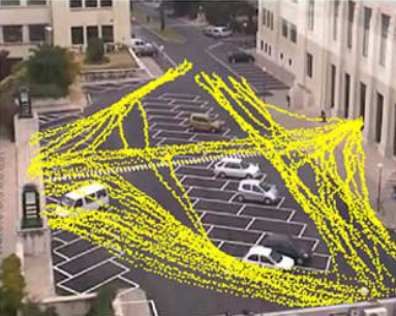
\includegraphics[height=2.2cm]{Figures/Nascimento-1}
			};
			\node at (-1.42,0) [draw=black,ultra thick,inner sep=0pt]
			{
				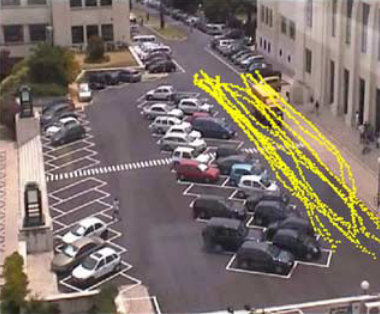
\includegraphics[height=2.2cm]{Figures/Nascimento-2}
			};
			\node at (0,-2.8) [draw=black,ultra thick,inner sep=0pt]
			{
				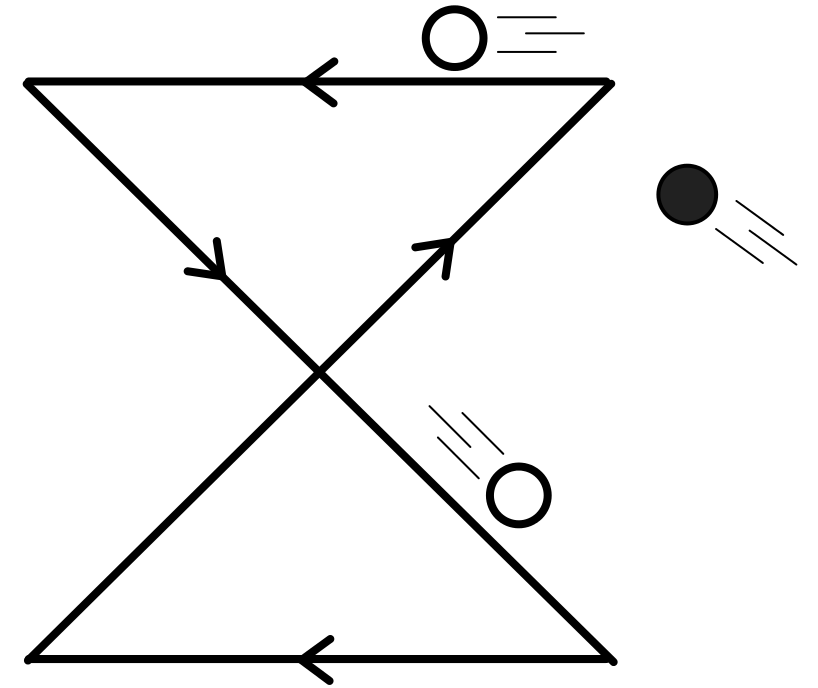
\includegraphics[width=3.6cm]{Figures/Veloso}
			};
		\end{tikzpicture}
	\end{columns}
	
	\vspace{0.47cm}
	
	\tiny
	
	\cite{Nascimento10} J. C. Nascimento \emph{et al.}, ``Trajectory classification using switched
	dynamical hidden Markov models'', Image Processing, 2010
	
	\cite{Vail07} D. L. Vail \emph{et al.}, ``Conditional random fields for activity recognition'',
	AAMAS, 2007 \\
\end{frame}

\begin{frame}
	\frametitle{PTracking}
	\framesubtitle{Distributed Particle Filtering for Multi-Sensor Multiple Object Tracking}
	
	\LARGE
	
	\begin{block}{Idea}
		Achieving \textbf{high} precision and robustness, as a global method does, while trying to keep
		a \textbf{low} computational load in order to obtain \textbf{real-time} performance, as
		recursive methods do
	\end{block}
\end{frame}

\begin{frame}
	\frametitle{PTracking}
	\framesubtitle{Contributions}
	
	\Large
	
	\vspace{0.2cm}
	
	We propose a novel technique based on \emph{Distributed Particle Filtering}. The key contributions
	are:
	
	\vspace{0.15cm}
	
	\begin{enumerate}
		\item \textbf{Real-time} multiple object tracking method
		\item Novel clustering method that \textbf{keeps} track of multiple objects whose number is
			  \textbf{not known} a priori, ensuring a \textbf{limited} Gaussian distribution in the
			  particle space
		\item \textbf{Asynchronous} algorithm to improve robustness with respect to communication
			  failures and dead nodes
	\end{enumerate}
\end{frame}

\begin{frame}
	\frametitle{PTracking}
	\framesubtitle{Group Tracking}
	
	\begin{figure}
		\begin{tikzpicture}[map/.style={draw=black,ultra thick,inner sep=0pt}]
			\node at (0,0) [map] {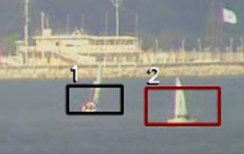
\includegraphics[width=0.32\linewidth]{Figures/GroupTracking-a}};
			\node at (4,0) [map] {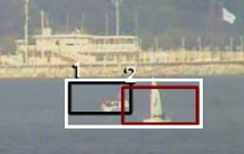
\includegraphics[width=0.32\linewidth]{Figures/GroupTracking-b}};
			\node at (8,0) [map] {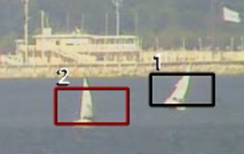
\includegraphics[width=0.32\linewidth]{Figures/GroupTracking-c}};
		\end{tikzpicture}
		\caption{Group tracking. Two sailing boats are going to cross each other. Occlusions are handled
				 considering the collapsing tracks to form a group, instead of tracking them
				 separately.}
	\end{figure}
\end{frame}

\begin{frame}
	\frametitle{KClusterize}
	\framesubtitle{Contributions}
	
	\Large
	
	\emph{KClusterize} has been designed aiming at fulfilling the following three requirements:
	
	\begin{enumerate}
		\item \textbf{Number} of objects to be detected \textbf{cannot} be known a priori
		\item \textbf{Low} computational load for real-time applications
		\item \textbf{Gaussian distribution} for each cluster
	\end{enumerate}
\end{frame}

\begin{frame}
	\frametitle{KClusterize}
	\framesubtitle{Cluster Gaussian Distribution}
	
	\setcounter{subfigure}{0}
	
	\begin{figure}[!t]
		\centering
		\subfigure[Output of the algorithm on frame \#269.]
		{
			\begin{tikzpicture}[map/.style={draw=black,ultra thick,inner sep=0pt}]
				\node at (0,0) [map]
				{
					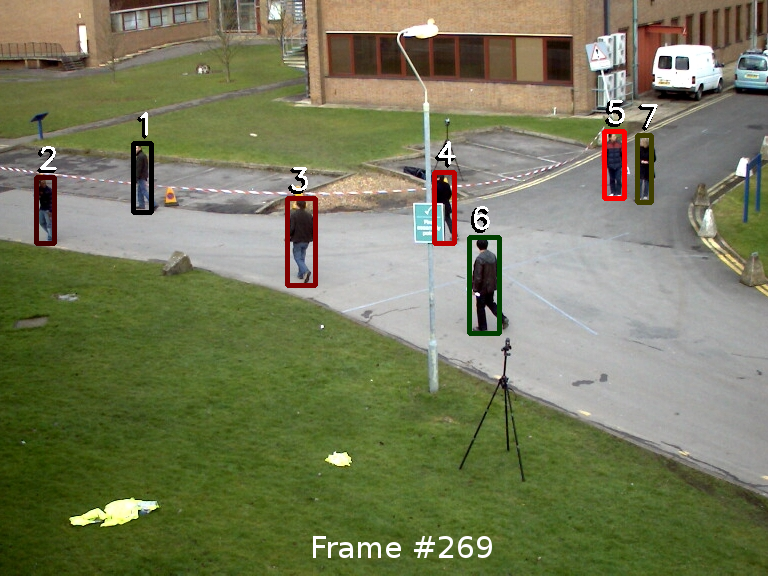
\includegraphics[width=0.48\linewidth]{Figures/KClusterize-Frame-0269-Output.png}
				};
			\end{tikzpicture}
		}
		\hspace{-3.8mm}
		\subfigure[A 2D visualization of frame \#269.]
		{
			\begin{tikzpicture}[map/.style={draw=white,ultra thick,inner sep=0pt}]
				\node at (0,0) [map]
				{
					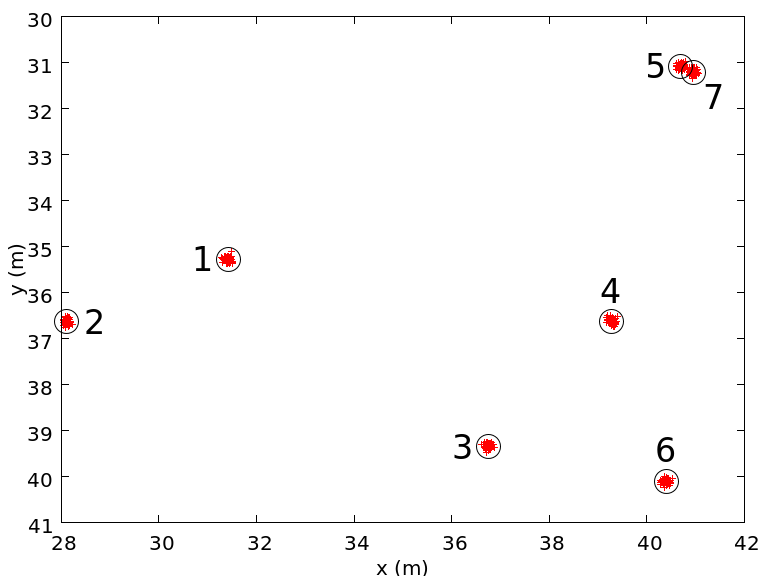
\includegraphics[width=0.48\linewidth]{Figures/KClusterize-Frame-0269-PlaneView.png}
				};
			\end{tikzpicture}
		}
	\end{figure}
\end{frame}

\begin{frame}
	\frametitle{Predicting Future Agent Motions}
	\framesubtitle{Contributions}
	
	\Large
	
	\vspace{0.4cm}
	
	We propose an integrated framework, which relies on \emph{PTracking}, for estimating future movement
	intentions of goal-oriented agents, that:
	
	\vspace{0.15cm}
	
	\begin{enumerate}
		\item \textbf{Does not} rely on semantic scene labelling
		\item \textbf{Incrementally} updates the IRL model over time
		\item Makes use of \textbf{non-uniform grids} for representing the state of the environment
	\end{enumerate}
\end{frame}

\begin{frame}
	\frametitle{Predicting Future Agent Motions}
	\framesubtitle{Observed Trajectory Extraction}
	
	\LARGE
	
	\vspace{0.4cm}
	
	We gather object estimates from \emph{PTracking} considering an arbitrary temporal window. \\
	
	\vspace{0.4cm}
	
	Having acquired a set of trajectories $ \mathcal{U} $, we \textbf{ground} each trajectory $ u \in
	\mathcal{U} $ in every policy $ \pi_s^G $. \\
\end{frame}

\begin{frame}
	\frametitle{Predicting Future Agent Motions}
	\framesubtitle{Goal Prediction}
	
	\Large
	
	\vspace{0.25cm}
	
	We \textbf{predict in real-time} the goal toward which each moving object is likely to be headed,
	by executing the policy that best matches its movement pattern.
	
	\vspace{-0.1cm}
	
	\begin{center}
		\begin{tikzpicture}
			\node at (0,0) [draw=black,ultra thick,inner sep=0pt]
			{
				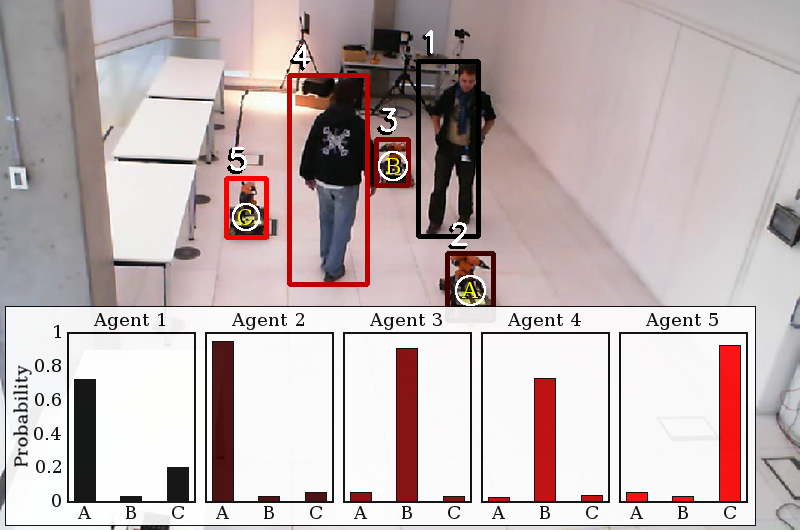
\includegraphics[width=0.59\linewidth]{Figures/Motivation}
			};
		\end{tikzpicture}
	\end{center}
\end{frame}

\begin{frame}
	\frametitle{Predicting Future Agent Motions}
	\framesubtitle{Anomaly Detection}
	
	\LARGE
	
	\vspace{0.5cm}
	
	It could happen that a trajectory $ u \in \mathcal{U} $ does not match any model:
	\begin{itemize}
		\item A trajectory fragment $ u $ is \textbf{anomalous} and refers to a \emph{suspicious
			  activity pattern}
		\item Environment has changed leading to new types of motion
			  \vspace{-0.25cm}
			  \begin{tabbing}
				  \hspace{0.3cm}
				  \large
				  $ \leadsto $ \emph{can be recognised by analysing the foreground model}
			  \end{tabbing}
	\end{itemize}
\end{frame}

\begin{frame}
	\frametitle{Challenge}
	
	\Large
	
	\vspace{0.25cm}
	
	\begin{figure}
		\centering
		\begin{tikzpicture}
			\node at (0,0) [draw=white,ultra thick,inner sep=0pt]
			{
				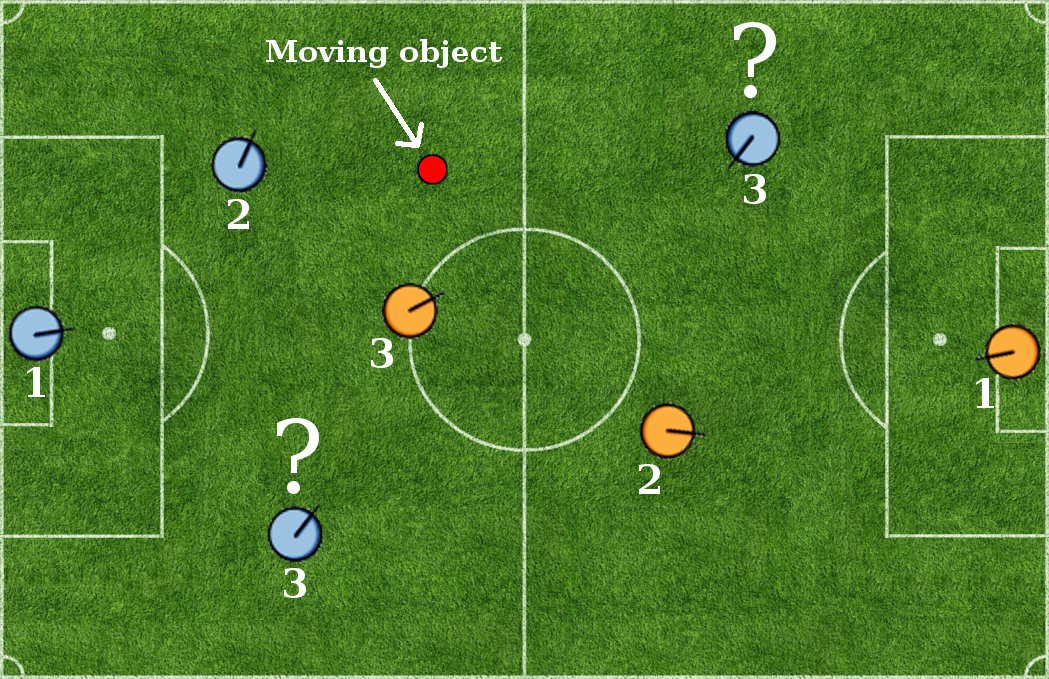
\includegraphics[width=0.8\linewidth]{Figures/Challenge}
			};
		\end{tikzpicture}
	\end{figure}
	
	\vspace{-0.4cm}
	
	\begin{center}
		What is the real position of the blue robot number 3?
	\end{center}
\end{frame}

\begin{frame}
	\frametitle{Quantitative Evaluation}
	\framesubtitle{RoboCup Domain}
	
	\large
	
	\vspace{-0.85cm}
	
	Simulating 3 Aldebaran Nao robots playing soccer, one of them alternatively forced to be inversely
	localised
	
	\Large
	
	\vspace{-0.6cm}
	
	\begin{columns}[T]
		\column{1.02\textwidth}
		
	\begin{figure}
		\centering
		
		\begin{tikzpicture}
			\node at (0,0) [draw=white,ultra thick,inner sep=0pt]
			{
				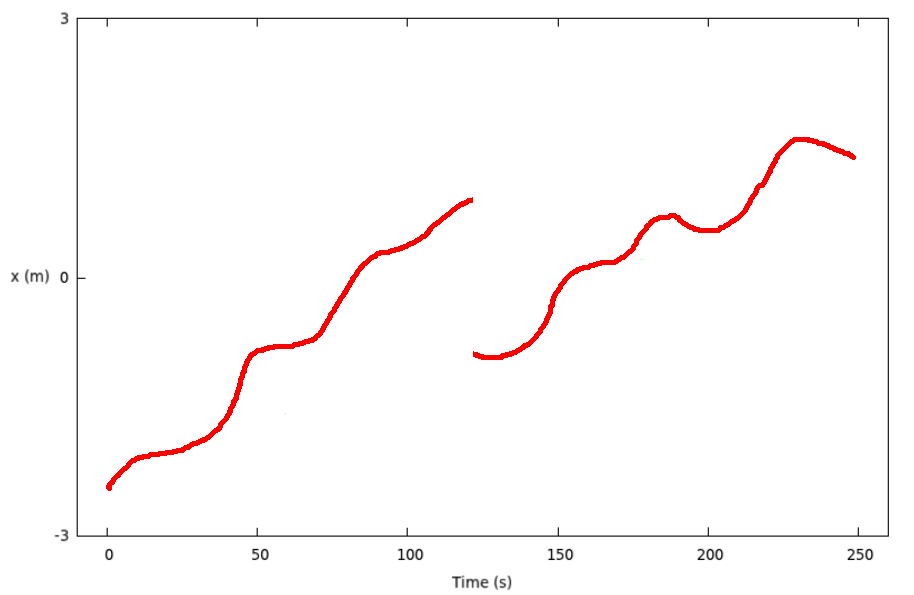
\includegraphics[width=0.34\linewidth]{Figures/Result-Scenario-2_Robot-1}
			};
			\node at (4.1,0) [draw=white,ultra thick,inner sep=0pt]
			{
				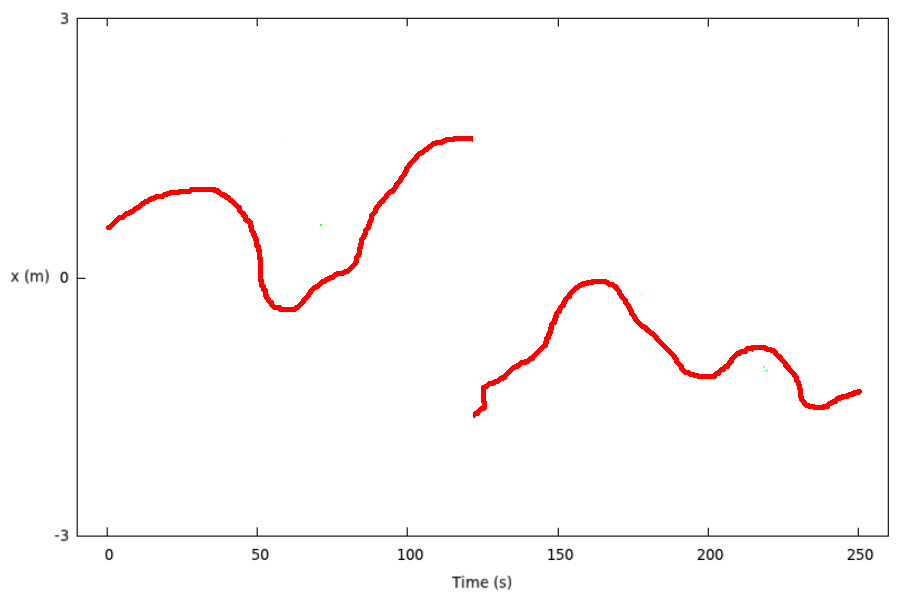
\includegraphics[width=0.34\linewidth]{Figures/Result-Scenario-2_Robot-2}
			};
			\node at (0,-2.9) [draw=white,ultra thick,inner sep=0pt]
			{
				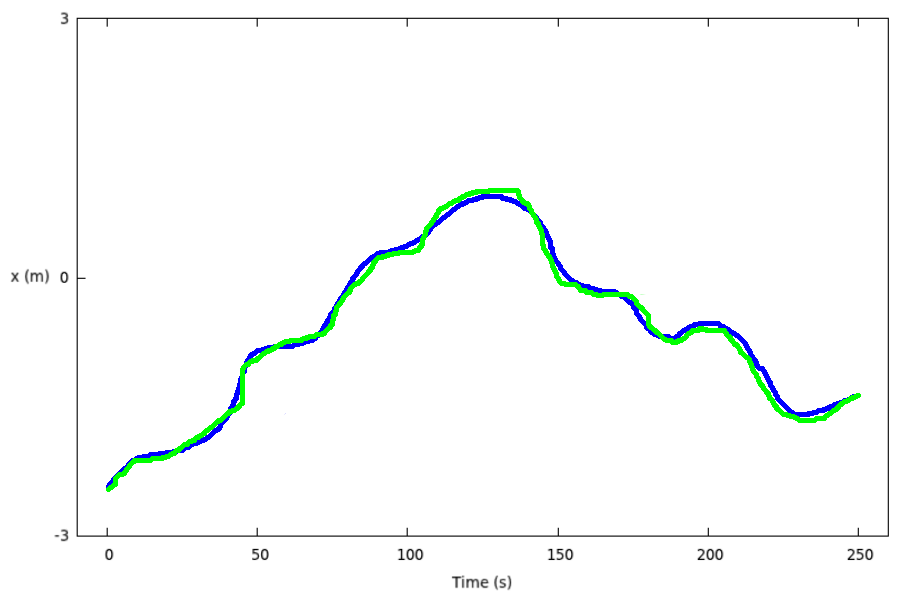
\includegraphics[width=0.34\linewidth]{Figures/Result-Scenario-2_Robot-1-GT}
			};
			\node at (4.1,-2.9) [draw=white,ultra thick,inner sep=0pt]
			{
				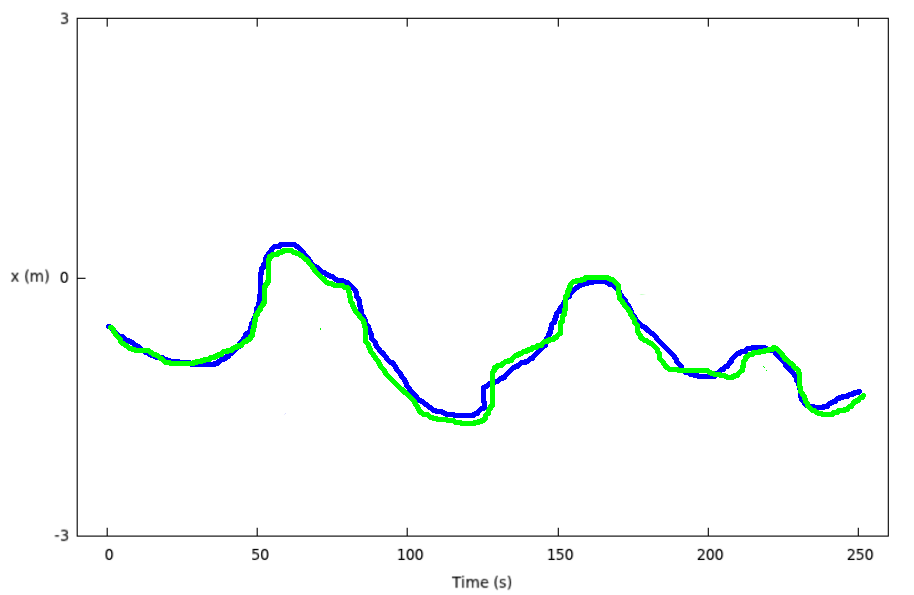
\includegraphics[width=0.34\linewidth]{Figures/Result-Scenario-2_Robot-2-GT}
			};
			\node at (8.2,0) [draw=white,ultra thick,inner sep=0pt]
			{
				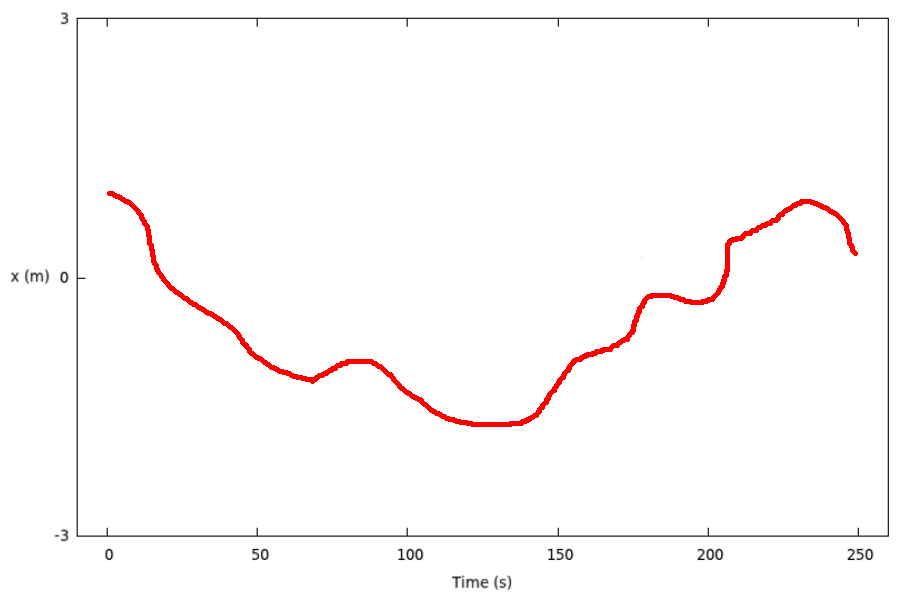
\includegraphics[width=0.34\linewidth]{Figures/Result-Scenario-2_Robot-3}
			};
			\node at (8.2,-2.9) [draw=white,ultra thick,inner sep=0pt]
			{
				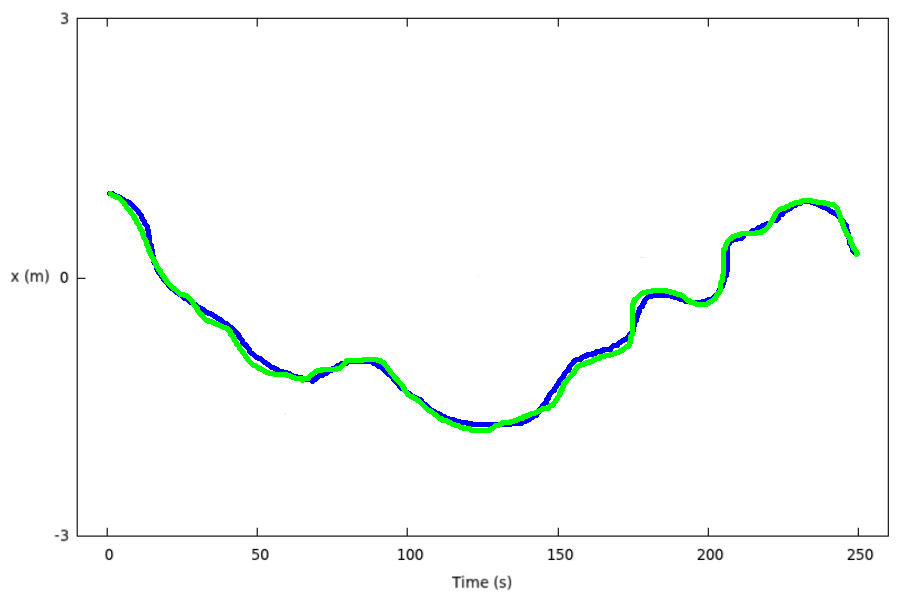
\includegraphics[width=0.34\linewidth]{Figures/Result-Scenario-2_Robot-3-GT}
			};
		\end{tikzpicture}
	\end{figure}
	\end{columns}
	
	\vspace{-6.15cm}
	
	\begin{tabbing}
		\hspace{0.21cm}
		\tiny
		\textbf{Robot 1 - Localization}
		\hspace{1.79cm}
		\textbf{Robot 2 - Localization}
		\hspace{1.79cm}
		\textbf{Robot 3 - Localization}
	\end{tabbing}
	
	\vspace{-1cm}
	
	\begin{tabbing}
		\hspace{0.4cm}
		\tiny
		\textcolor{blue}{Correctly}
	\end{tabbing}
	
	\vspace{-1.2cm}
	
	\begin{tabbing}
		\hspace{0.42cm}
		\tiny
		\textcolor{blue}{localized}
	\end{tabbing}
	
	\vspace{-1.17cm}
	
	\begin{tabbing}
		\footnotesize
		\hspace{0.87cm}
		\textcolor{blue}{$ \searrow $}
	\end{tabbing}
	
	\vspace{-1.43cm}
	
	\begin{tabbing}
		\footnotesize
		\hspace{2.68cm}
		\textcolor{blue}{$ \nwarrow $}
	\end{tabbing}
	
	\vspace{-1.2cm}
	
	\begin{tabbing}
		\hspace{2.53cm}
		\tiny
		\textcolor{blue}{Wrongly}
	\end{tabbing}
	
	\vspace{-1.2cm}
	
	\begin{tabbing}
		\hspace{2.52cm}
		\tiny
		\textcolor{blue}{localized}
	\end{tabbing}
	
	\vspace{-1.83cm}
	
	\begin{tabbing}
		\footnotesize
		\hspace{4.8cm}
		\textcolor{blue}{$ \nearrow $}
	\end{tabbing}
	
	\vspace{-1.2cm}
	
	\begin{tabbing}
		\hspace{4.35cm}
		\tiny
		\textcolor{blue}{Wrongly}
	\end{tabbing}
	
	\vspace{-1.2cm}
	
	\begin{tabbing}
		\hspace{4.34cm}
		\tiny
		\textcolor{blue}{localized}
	\end{tabbing}
	
	\vspace{-2.75cm}
	
	\begin{tabbing}
		\hspace{6.82cm}
		\tiny
		\textcolor{blue}{Correctly}
	\end{tabbing}
	
	\vspace{-1.2cm}
	
	\begin{tabbing}
		\hspace{6.84cm}
		\tiny
		\textcolor{blue}{localized}
	\end{tabbing}
	
	\vspace{-1.17cm}
	
	\begin{tabbing}
		\footnotesize
		\hspace{7cm}
		\textcolor{blue}{$ \swarrow $}
	\end{tabbing}
	
	\vspace{-1.79cm}
	
	\begin{tabbing}
		\hspace{9.52cm}
		\tiny
		\textcolor{blue}{Correctly}
	\end{tabbing}
	
	\vspace{-1.2cm}
	
	\begin{tabbing}
		\hspace{9.54cm}
		\tiny
		\textcolor{blue}{localized}
	\end{tabbing}
	
	\vspace{-1.17cm}
	
	\begin{tabbing}
		\footnotesize
		\hspace{9.99cm}
		\textcolor{blue}{$ \searrow $}
	\end{tabbing}
	
	\vspace{0.01cm}
	
	\begin{tabbing}
		\hspace{0.21cm}
		\tiny
		\textbf{Robot 1 - Filtered vs Ground-Truth}
		\hspace{0.53cm}
		\textbf{Robot 2 - Filtered vs Ground-Truth}
		\hspace{0.53cm}
		\textbf{Robot 3 - Filtered vs Ground-Truth}
	\end{tabbing}
\end{frame}

\begin{frame}
	\frametitle{Qualitative Evaluation}
	\framesubtitle{RoboCup Iran Open}
	
	\begin{figure}[!h]
		\centering
		\includemovie[inline=false,text=
		{
			\begin{tikzpicture}
				\node at (0,0) [draw=black,ultra thick,inner sep=0pt]
				{
					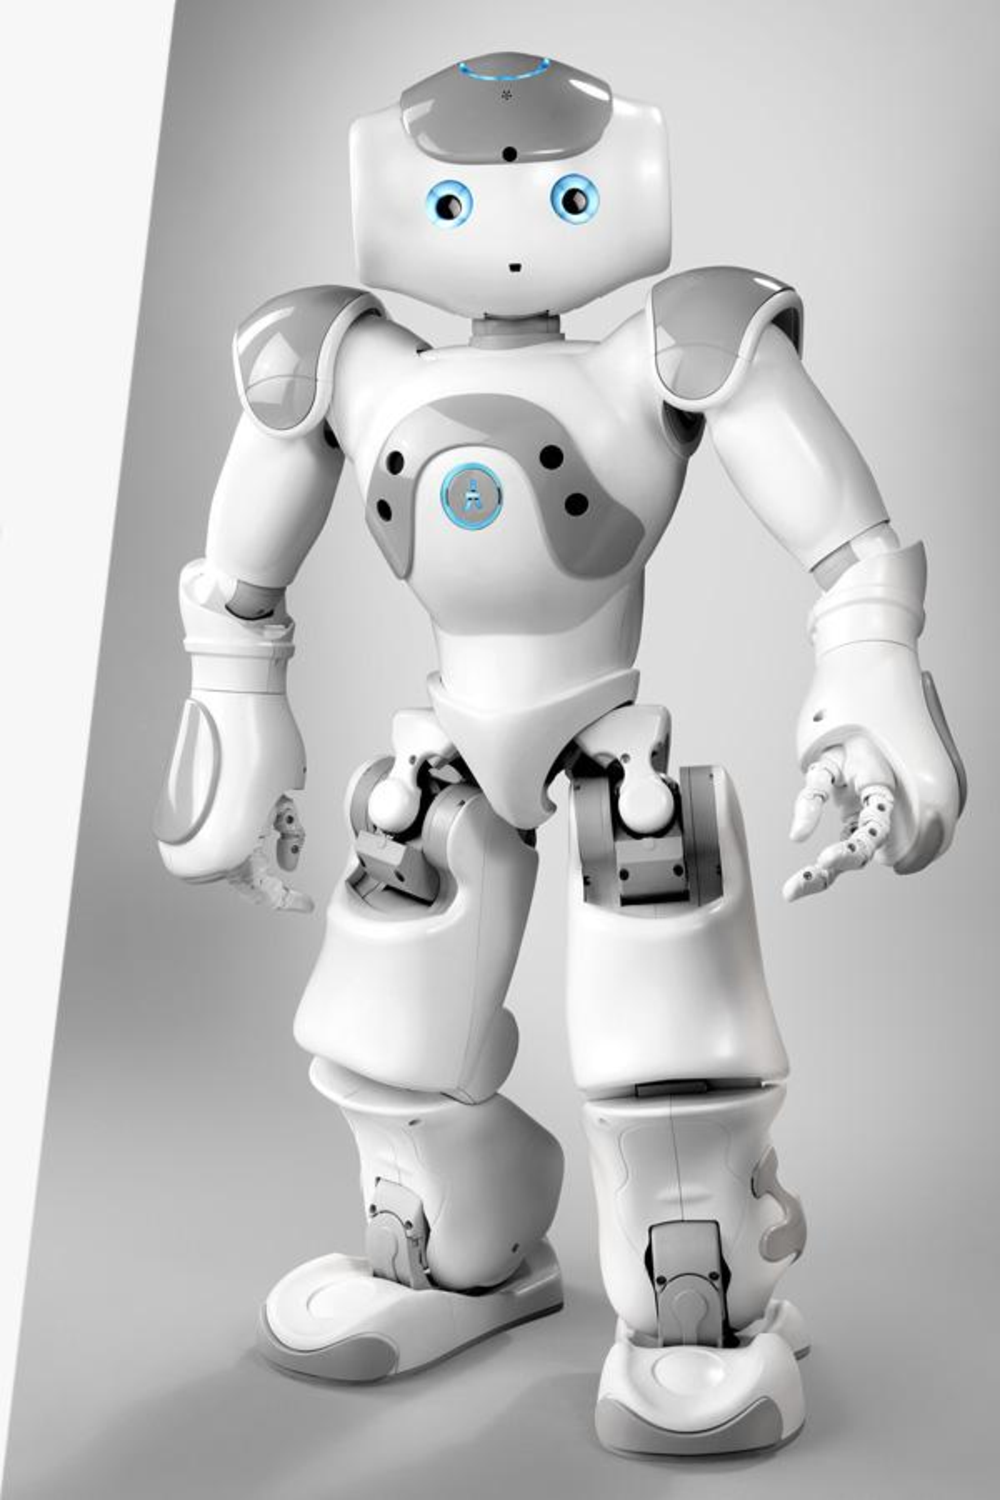
\includegraphics[width=0.85\linewidth]{Figures/Nao}
				};
			\end{tikzpicture}
		}]{}{}{../Videos/2-Nao/PTracking-RLSD.avi}
	\end{figure}
\end{frame}

\begin{frame}
	\frametitle{Qualitative Evaluation}
	\framesubtitle{Maritime Domain - Blue Water}
	
	\begin{figure}[!h]
		\centering
		\includemovie[inline=false,text=
		{
			\begin{tikzpicture}
				\node at (0,0) [draw=black,ultra thick,inner sep=0pt]
				{
					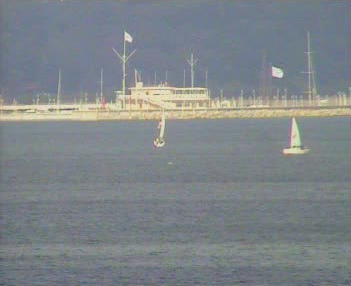
\includegraphics[width=0.65\linewidth]{Figures/Boat-2}
				};
			\end{tikzpicture}
		}]{}{}{../Videos/1-Boat/PTracking-Wester_LLTV_VELA.avi}
	\end{figure}
\end{frame}

\begin{frame}
	\frametitle{Experimental Evaluation}
	\framesubtitle{Multi-Sensor, Multi-Object}
	
	\large
	
	\vspace{-0.35cm}
	
	\begin{columns}[t]
		\only<1->
		{
			\column{0.8\textwidth}
			
			\begin{block}{Issia Soccer}
				tracking of players in a real soccer match
			\end{block}
			
			\column{0.15\textwidth}
		}
	\end{columns}
	
	\begin{center}
		\begin{tikzpicture}
			\node at (2.39,0) [draw=black,ultra thick,inner sep=0pt]  {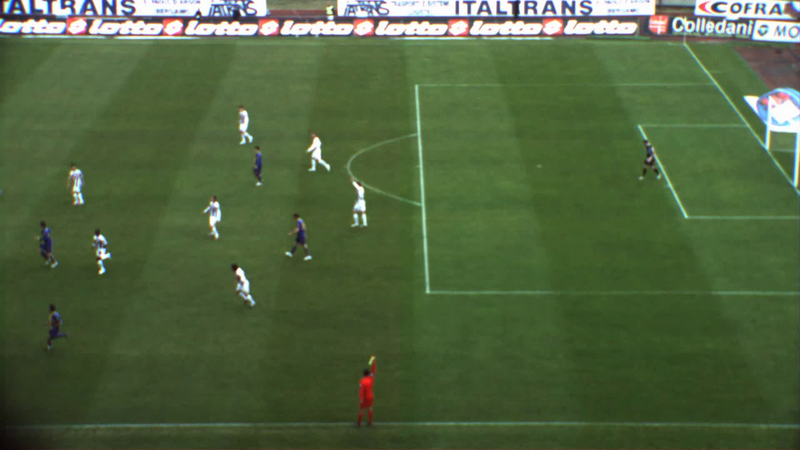
\includegraphics[height=2.1cm]{Figures/IssiaSoccer-Camera1}};
			\node at (6.26,0) [draw=black,ultra thick,inner sep=0pt]  {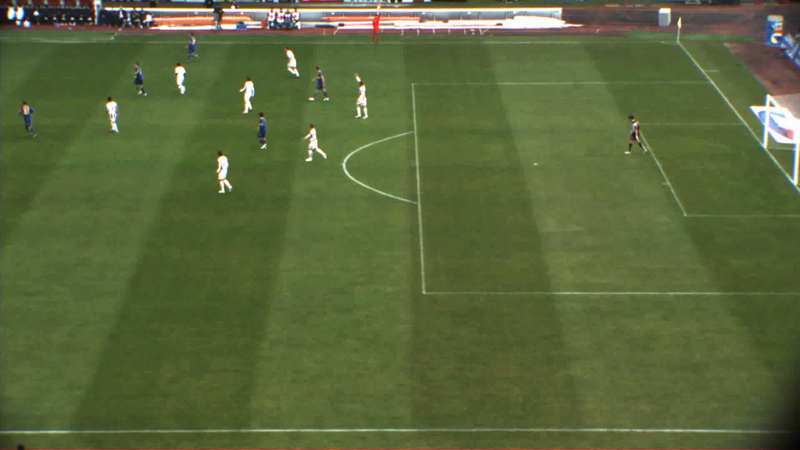
\includegraphics[height=2.1cm]{Figures/IssiaSoccer-Camera2}};
			\node at (2.39,-2.22) [draw=black,ultra thick,inner sep=0pt]  {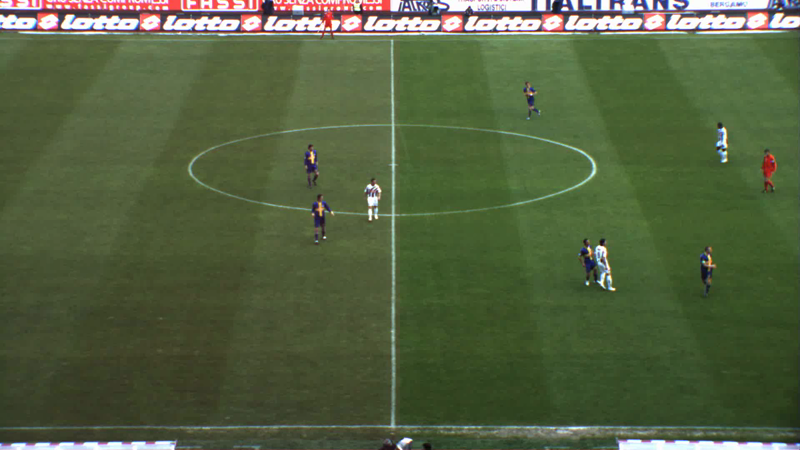
\includegraphics[height=2.1cm]{Figures/IssiaSoccer-Camera3}};
			\node at (6.26,-2.22) [draw=black,ultra thick,inner sep=0pt]  {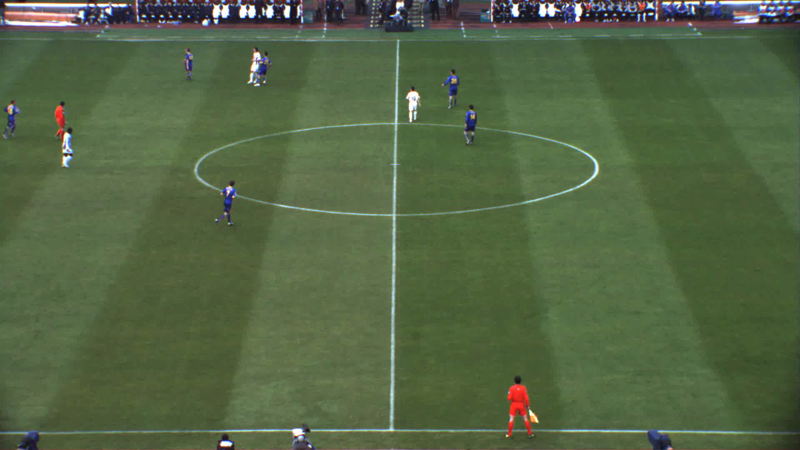
\includegraphics[height=2.1cm]{Figures/IssiaSoccer-Camera4}};
		\end{tikzpicture}
	\end{center}
	
	\vspace{-0.05cm}
	
	\tiny
	
	\textbf{A Distributed Approach for Real-Time Multi-Camera Multi-Object Tracking} \\
	F. Previtali, D. D. Bloisi, L. Iocchi \\
	\emph{Journal on Machine Vision and Applications} [submitted] \\
\end{frame}

\begin{frame}
	\frametitle{Quantitative Evaluation}
	\framesubtitle{People Domain - Issia Soccer}
	
	\Large
	
	\begin{table}[!t]
		\renewcommand{\arraystretch}{1.3}
		\centering
		\begin{tabular}{lcccc}
			\hline
			\hline
			\multicolumn{1}{c}{\begin{tabular}[c]{@{}c@{}}\textbf{Method} \end{tabular}} & \textbf{MOTA} & \textbf{MOTP} \\
			\hline
			PTracking - Camera 1 & 0.723 & 0.612 \\
			\hline
			PTracking - Camera 1, 2 & 0.789 & 0.638 \\
			\hline
			PTracking - Camera 1, 2, 3 & 0.817 & 0.651 \\
			\hline
			PTracking - Camera 1, 2, 3, 4 & 0.894 & 0.706 \\
			\hline
		\hline
		\end{tabular}
	\end{table}
\end{frame}

\begin{frame}
	\frametitle{Qualitative Evaluation}
	\framesubtitle{People Domain - Issia Soccer}
	
	\begin{figure}[!h]
		\centering
		\includemovie[inline=false,text=
		{
			\begin{tikzpicture}
				\node at (0,0) [draw=black,ultra thick,inner sep=0pt]
				{
					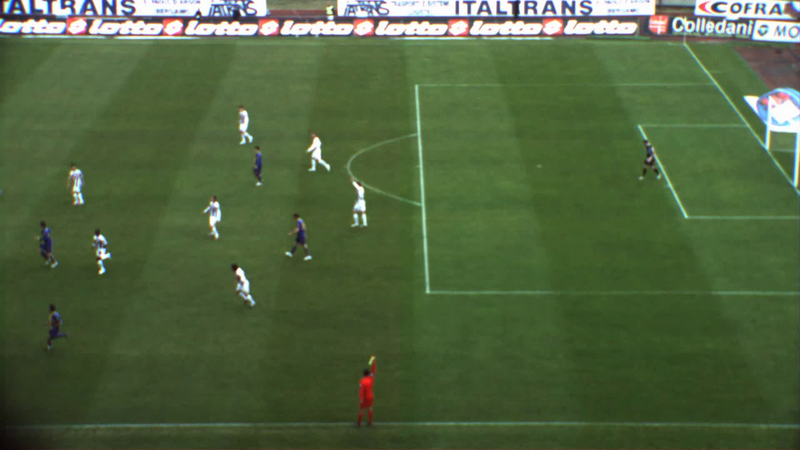
\includegraphics[width=0.85\linewidth]{Figures/IssiaSoccer-Camera1}
				};
			\end{tikzpicture}
		}]{}{}{../Videos/4-People/PTracking-IssiaSoccer.mp4}
	\end{figure}
\end{frame}

\begin{frame}
	\frametitle{Experimental Evaluation}
	\framesubtitle{Multi-Sensor, Multi-Object}
	
	\large
	
	\vspace{-0.45cm}
	
	\begin{columns}[t]
		\only<1->
		{
			\column{0.8\textwidth}
			
			\begin{block}{PETS-2009}
				tracking of individuals within a crowd
			\end{block}
			
			\column{0.15\textwidth}
		}
	\end{columns}
	
	\vspace{0.1cm}
	
	\begin{center}
		\begin{tikzpicture}
			\node at (0,0) [draw=black,ultra thick,inner sep=0pt]  {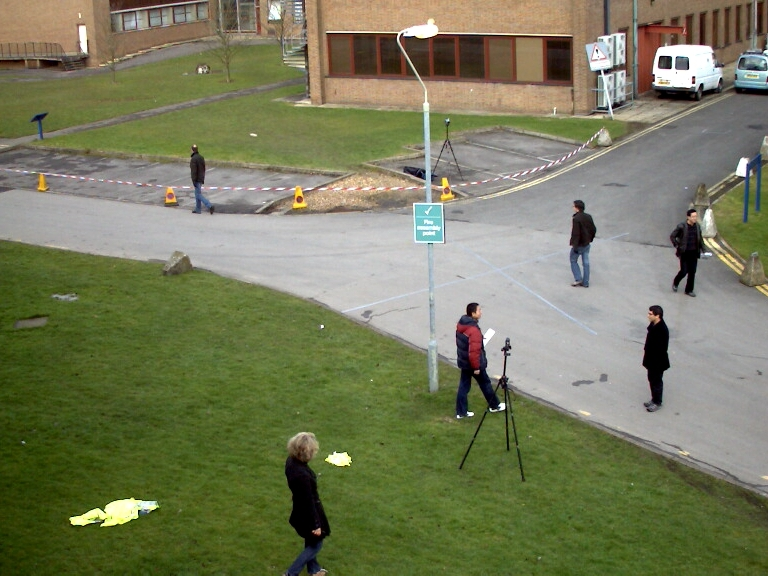
\includegraphics[height=2.55cm]{Figures/PETS2009-1}};
			\node at (3.55,0) [draw=black,ultra thick,inner sep=0pt]  {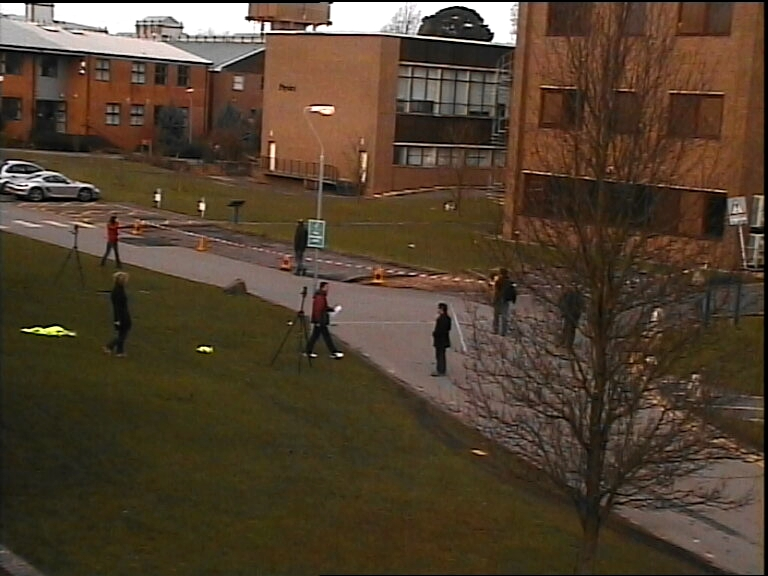
\includegraphics[height=2.55cm]{Figures/PETS2009-3}};
			\node at (7.17,0) [draw=black,ultra thick,inner sep=0pt]  {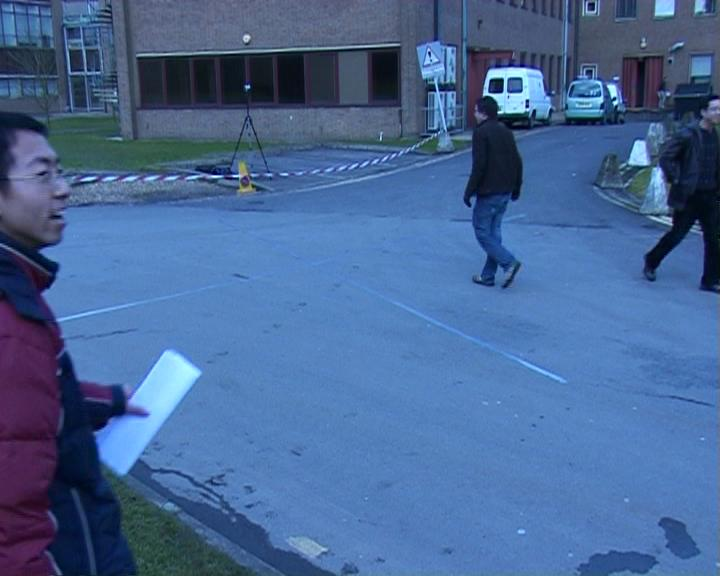
\includegraphics[height=2.55cm]{Figures/PETS2009-6}};
			\node at (1.8,-2.7) [draw=black,ultra thick,inner sep=0pt]  {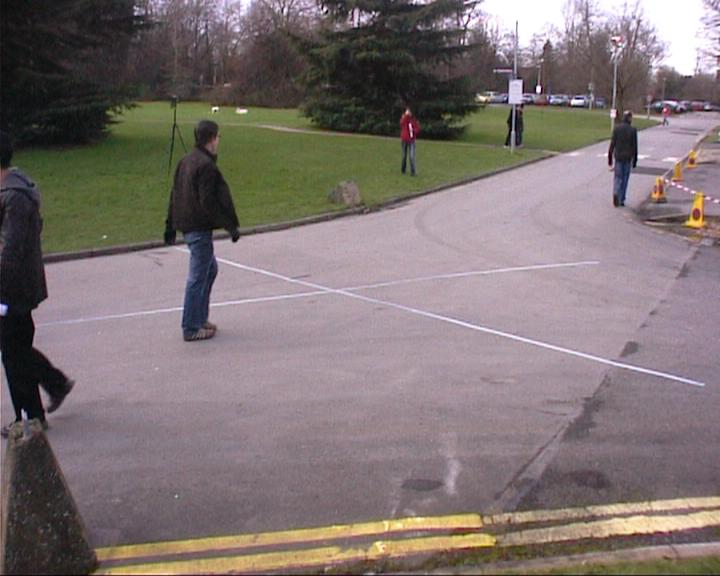
\includegraphics[height=2.55cm]{Figures/PETS2009-7}};
			\node at (5.5,-2.7) [draw=black,ultra thick,inner sep=0pt]  {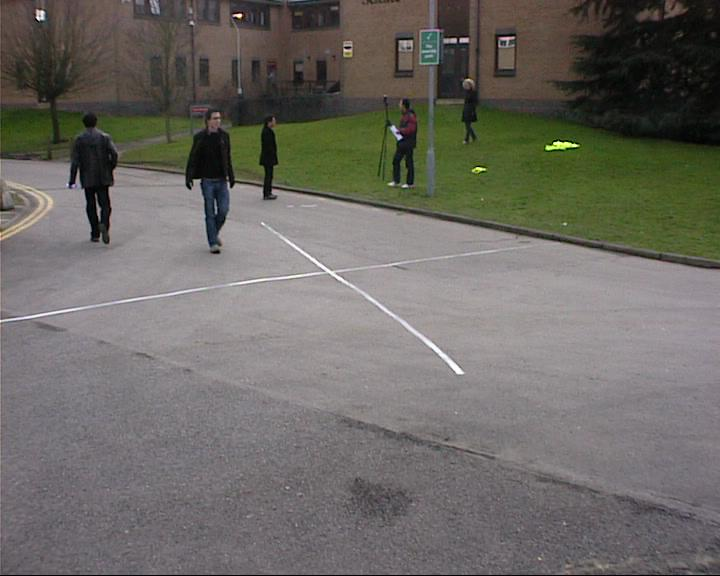
\includegraphics[height=2.55cm]{Figures/PETS2009-8}};
		\end{tikzpicture}
	\end{center}
\end{frame}

\begin{frame}
	\frametitle{Quantitative Evaluation}
	\framesubtitle{People Domain - PETS-2009}
	
	\large
	
	\begin{table}[!t]
		\renewcommand{\arraystretch}{1.3}
		\centering
		\begin{tabular}{ccccc}
			\hline
			\hline
			\textbf{Method} & \textbf{MOTA} & \textbf{MOTP} & \textbf{Type} & \textbf{Real-Time} \\
			\hline
			Leal-Taix\'{e} \cite{Leal11} & 0.67 & 0.534 & OFFLINE & NO \\
			\hline
			Berclaz \cite{Berclaz11} & 0.732 & 0.603 & OFFLINE & NO \\
			\hline
			Henriques \cite{Henriques11} & 0.833 & 0.711 & OFFLINE & NO \\
			\hline
			Breitenstein \cite{Breitenstein11} & 0.745 & 0.563 & ONLINE & NO \\
			\hline
			Yang \cite{Yang09} & 0.759 & 0.538 & ONLINE & NO \\
			\hline
			Bae \cite{Bae14} & 0.830 & 0.696 & ONLINE & \textbf{YES} \\
			\hline
			PTracking & \textbf{0.874} & \textbf{0.722} & ONLINE & \textbf{YES (30.2 FPS)} \\
			\hline
			PTracking$^*$ & \textbf{0.882} & \textbf{0.717} & ONLINE & NO (11.8 FPS) \\
			\hline
		\hline
		\end{tabular}
	\end{table}
\end{frame}

\begin{frame}
	\frametitle{Experimental Evaluation}
	\framesubtitle{Multi-Sensor, Multi-Object}
	
	\large
	
	\begin{columns}[t]
		\only<1->
		{
			\column{0.8\textwidth}
			
			\begin{block}{Prey-Predator Game}
				demonstrating the advantages of using mobile sensors
			\end{block}
			
			\column{0.15\textwidth}
		}
	\end{columns}
	
	\vspace{0.1cm}
	
	\begin{center}
		\begin{tikzpicture}
			\node at (0,0) [draw=black,ultra thick,inner sep=0pt]  {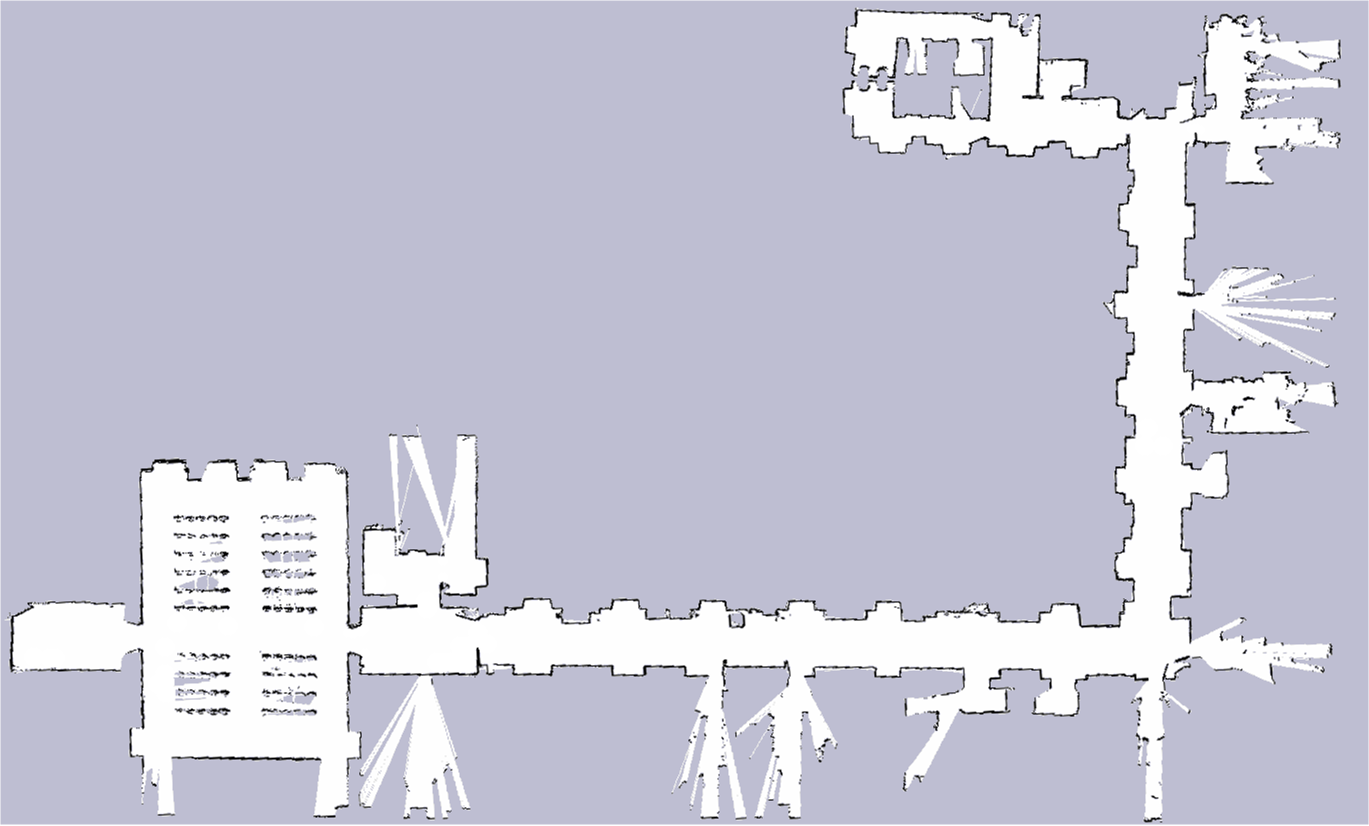
\includegraphics[height=3.25cm]{Figures/Map-1}};
			\node at (6,0) [draw=black,ultra thick,inner sep=0pt]  {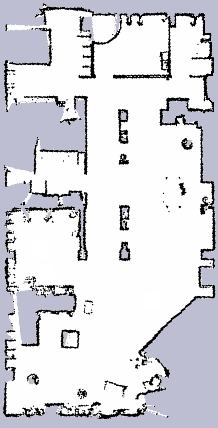
\includegraphics[height=3.25cm]{Figures/Map-2}};
		\end{tikzpicture}
	\end{center}
	
	\vspace{0.52cm}
	
	\tiny
	
	\textbf{PTracking: Distributed Multi-Agent Multi-Object Tracking through Multi-Clustered Particle
	Filtering} \\
	F. Previtali, L. Iocchi \\
	\emph{IEEE International Conference on Multisensor Fusion and Integration for Intelligent Systems,
	2015} \\
\end{frame}

\begin{frame}
	\frametitle{Quantitative Evaluation}
	\framesubtitle{DIAG}
	
	\small
	
	\begin{table}[!t]
		\centering
		\begin{tabular}{ccccc}
			\cline{1-5}
			\multicolumn{1}{l}{} & \multicolumn{4}{c}{\textbf{\begin{tabular}[c]{@{}c@{}}
			Prey-Predator Distance (avg $ \pm $ std. dev.)\end{tabular}}} \\ \hline
			\multicolumn{1}{c}{\textbf{\#}} & \textbf{Setting 1} & \textbf{Setting 2} &
			\textbf{Setting 3} & \textbf{Setting 4} \\
			
			\multicolumn{1}{c}{1} & 3.04 $ \pm $ 0.63 $ m $ & 2.70 $ \pm $ 0.49
								  $ m $ & 2.02 $ \pm $ 0.38 $ m $ & 1.12 $ \pm $
								  0.19 $ m $ \\
			\multicolumn{1}{c}{2} & 2.95 $ \pm $ 0.80 $ m $ & 2.65 $ \pm $ 0.48
								  $ m $ & 1.95 $ \pm $ 0.42 $ m $ & 1.15 $ \pm $
								  0.20 $ m $ \\
			\multicolumn{1}{c}{3} & 3.12 $ \pm $ 0.53 $ m $ & 2.87 $ \pm $ 0.56
								  $ m $ & 2.03 $ \pm $ 0.41 $ m $ & 1.13 $ \pm $
								  0.19 $ m $ \\
			\multicolumn{1}{c}{4} & 3.01 $ \pm $ 0.69 $ m $ & 2.73 $ \pm $ 0.49
								  $ m $ & 2.06 $ \pm $ 0.38 $ m $ & 1.08 $ \pm $
								  0.22 $ m $ \\
			\multicolumn{1}{c}{5} & 2.99 $ \pm $ 0.72 $ m $ & 2.86 $ \pm $ 0.61
								  $ m $ & 1.99 $ \pm $ 0.40 $ m $ & 1.11 $ \pm $
								  0.17 $ m $ \\
			\hline
			
			\\
			
			\hline
			\multicolumn{1}{l}{} & \multicolumn{4}{c}{\textbf{\begin{tabular}[c]
			{@{}c@{}}Tracking Performance (MOTA,MOTP)\end{tabular}}} \\ \hline
			\multicolumn{1}{c}{\textbf{\#}} & \textbf{Setting 1} & \textbf{Setting 2} &
			\textbf{Setting 3} & \textbf{Setting 4} \\
			
			\multicolumn{1}{c}{1} & (0.63,0.45) & (0.67,0.49) & (0.75,0.51) & (0.94,0.75) \\
			\multicolumn{1}{c}{2} & (0.59,0.42) & (0.65,0.45) & (0.73,0.49) & (0.92,0.74) \\
			\multicolumn{1}{c}{3} & (0.64,0.41) & (0.69,0.48) & (0.70,0.47) & (0.95,0.77) \\
			\multicolumn{1}{c}{4} & (0.62,0.45) & (0.62,0.40) & (0.74,0.50) & (0.92,0.75) \\
			\multicolumn{1}{c}{5} & (0.57,0.39) & (0.64,0.44) & (0.70,0.48) & (0.94,0.77) \\
			\hline
		\end{tabular}
	\end{table}
\end{frame}

\begin{frame}
	\frametitle{Quantitative Evaluation}
	\framesubtitle{Peccioli House}
	
	\small
	
	\begin{table}
		\centering
		\begin{tabular}{ccccc}
			\cline{1-5}
			\multicolumn{1}{l}{} & \multicolumn{4}{c}{\textbf{\begin{tabular}[c]{@{}c@{}}
			Prey-Predator Distance (avg $ \pm $ std. dev.)\end{tabular}}} \\ \hline
			\multicolumn{1}{c}{\textbf{\#}} & \textbf{Setting 1} & \textbf{Setting 2} &
			\textbf{Setting 3} & \textbf{Setting 4} \\
			
			\multicolumn{1}{c}{1} & 2.84 $ \pm $ 0.59 $ m $ & 2.55 $ \pm $ 0.47
								  $ m $ & 1.85 $ \pm $ 0.38 $ m $ & 1.07 $ \pm $
								  0.18 $ m $ \\
			\multicolumn{1}{c}{2} & 2.85 $ \pm $ 0.74 $ m $ & 2.52 $ \pm $ 0.51
								  $ m $ & 1.84 $ \pm $ 0.40 $ m $ & 1.05 $ \pm $
								  0.21 $ m $ \\
			\multicolumn{1}{c}{3} & 3.03 $ \pm $ 0.57 $ m $ & 2.76 $ \pm $ 0.52
								  $ m $ & 1.91 $ \pm $ 0.43 $ m $ & 1.11 $ \pm $
								  0.20 $ m $ \\
			\multicolumn{1}{c}{4} & 3.04 $ \pm $ 0.61 $ m $ & 2.63 $ \pm $ 0.47
								  $ m $ & 1.93 $ \pm $ 0.39 $ m $ & 1.08 $ \pm $
								  0.21 $ m $ \\
			\multicolumn{1}{c}{5} & 2.89 $ \pm $ 0.68 $ m $ & 2.77 $ \pm $ 0.56
								  $ m $ & 1.89 $ \pm $ 0.41 $ m $ & 1.09 $ \pm $
								  0.15 $ m $ \\
			
			\hline
			
			\\
			
			\hline
			\multicolumn{1}{l}{} & \multicolumn{4}{c}{\textbf{\begin{tabular}[c]
			{@{}c@{}}Tracking Performance (MOTA,MOTP)\end{tabular}}} \\ \hline
			\multicolumn{1}{c}{\textbf{\#}} & \textbf{Setting 1} & \textbf{Setting 2} &
			\textbf{Setting 3} & \textbf{Setting 4} \\
			
			\multicolumn{1}{c}{1} & (0.67,0.42) & (0.71,0.49) & (0.78,0.58) & (0.93,0.79) \\
			\multicolumn{1}{c}{2} & (0.62,0.43) & (0.69,0.46) & (0.77,0.55) & (0.95,0.76) \\
			\multicolumn{1}{c}{3} & (0.64,0.47) & (0.73,0.51) & (0.72,0.52) & (0.96,0.79) \\
			\multicolumn{1}{c}{4} & (0.66,0.44) & (0.68,0.43) & (0.75,0.53) & (0.93,0.77) \\
			\multicolumn{1}{c}{5} & (0.60,0.41) & (0.65,0.45) & (0.71,0.51) & (0.97,0.81) \\
			\hline
		\end{tabular}
	\end{table}
\end{frame}

\begin{frame}
	\frametitle{Qualitative Evaluation}
	\framesubtitle{InSpace}
	
	\begin{figure}[!h]
		\centering
		\includemovie[inline=false,text=
		{
			\begin{tikzpicture}
				\node at (0,0) [draw=black,ultra thick,inner sep=0pt]
				{
					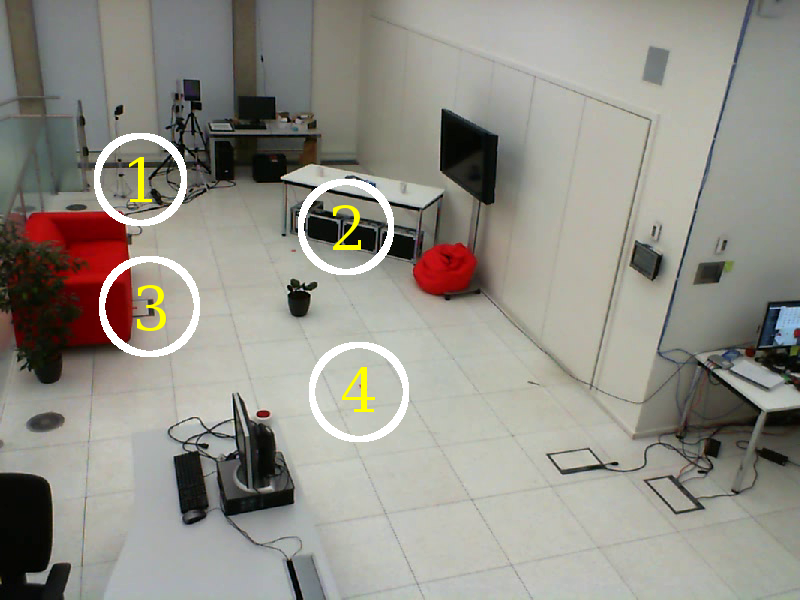
\includegraphics[width=0.65\linewidth]{Figures/InSpace_FrontCamera_Goals}
				};
			\end{tikzpicture}
		}]{}{}{../Videos/5-ActivityForecasting/PTracking-House.avi}
	\end{figure}
\end{frame}

\begin{frame}
	\frametitle{Experimental Evaluation}
	\framesubtitle{Interactive Costmaps}
	
	\large
	
	\begin{columns}[t]
		\only<1->
		{
			\column{0.8\textwidth}
			
			\begin{block}{Effective Social Motion Planning}
				reasoning about interactive agents' intention in the environment in order to adapt the
				costmap over time
			\end{block}
			
			\column{0.15\textwidth}
		}
	\end{columns}
	
	\vspace{0.2cm}
	
	\begin{center}
		\begin{tikzpicture}
			\node at (0,0) [draw=black,ultra thick,inner sep=0pt]  {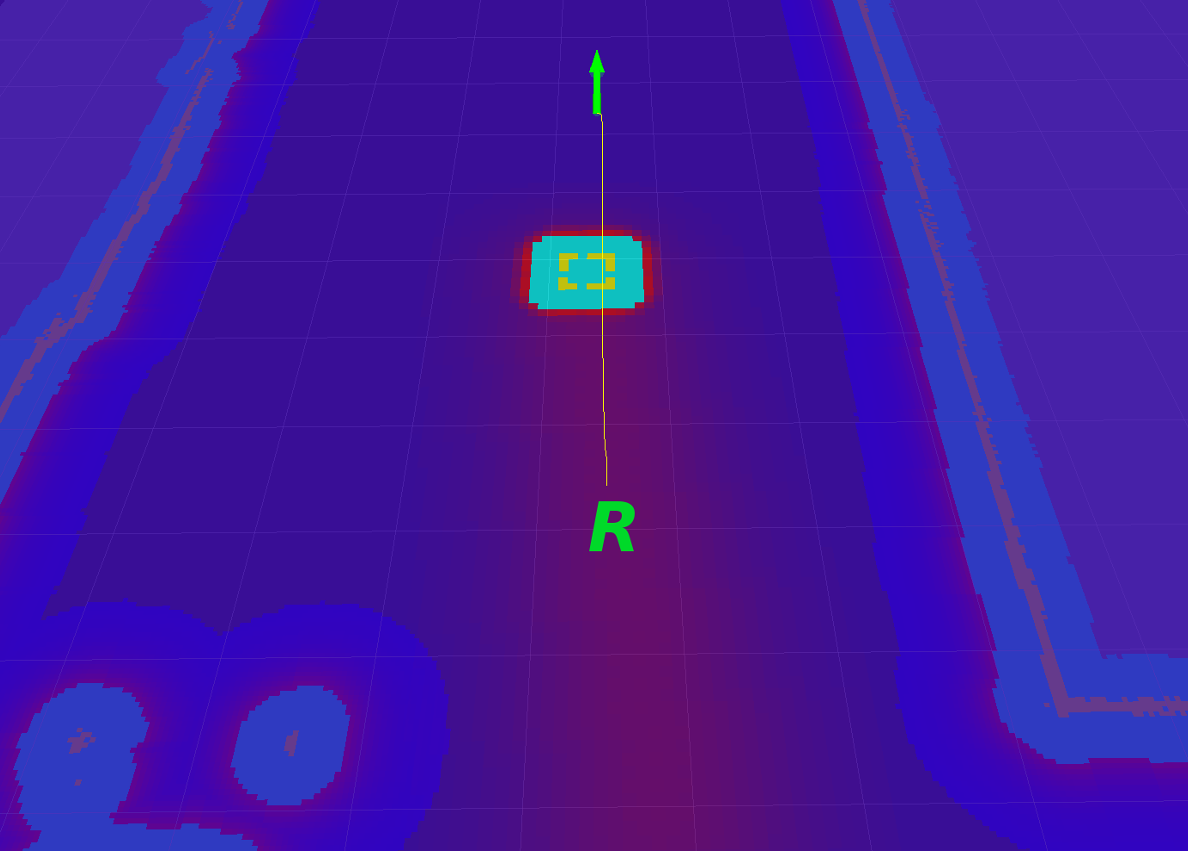
\includegraphics[height=2.8cm]{Figures/ConstantVelocityComparison}};
			\node at (4.05,0) [draw=black,ultra thick,inner sep=0pt]  {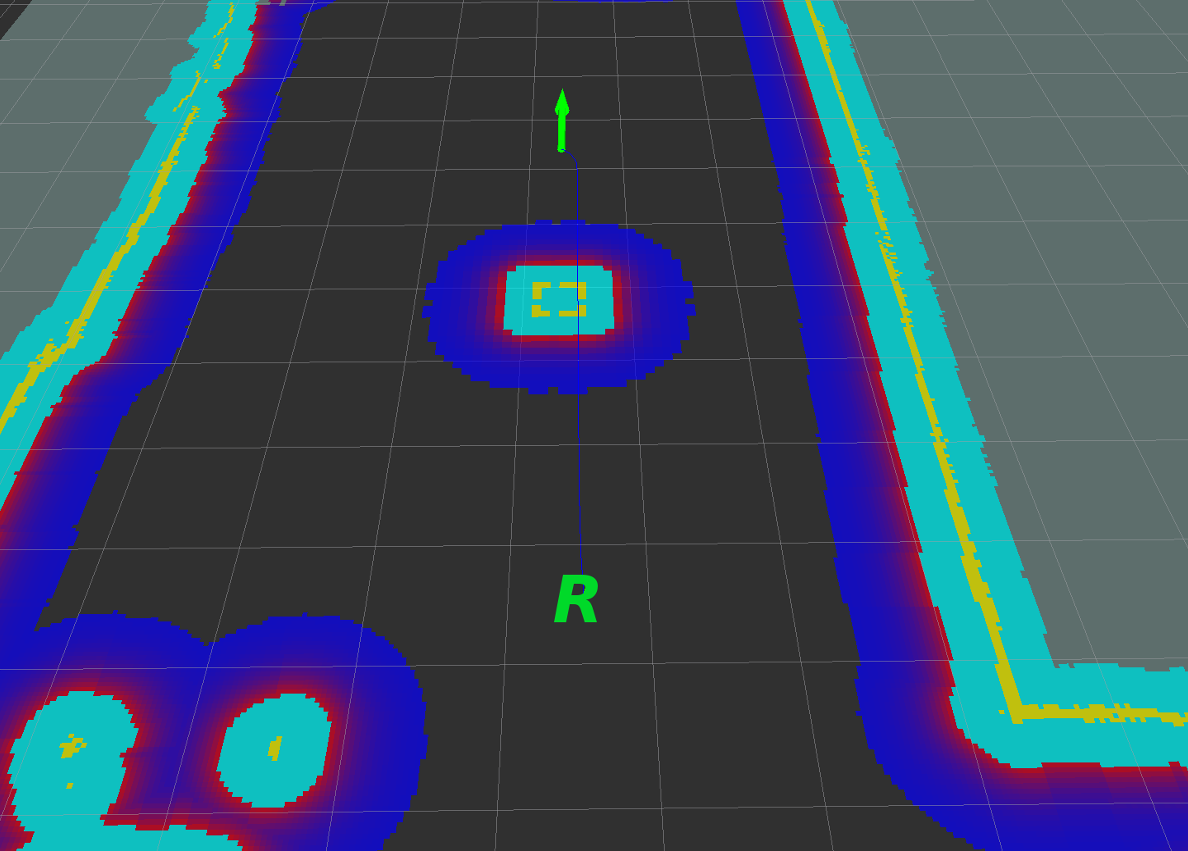
\includegraphics[height=2.8cm]{Figures/ProxemicsComparison}};
			\node at (8.11,0) [draw=black,ultra thick,inner sep=0pt]  {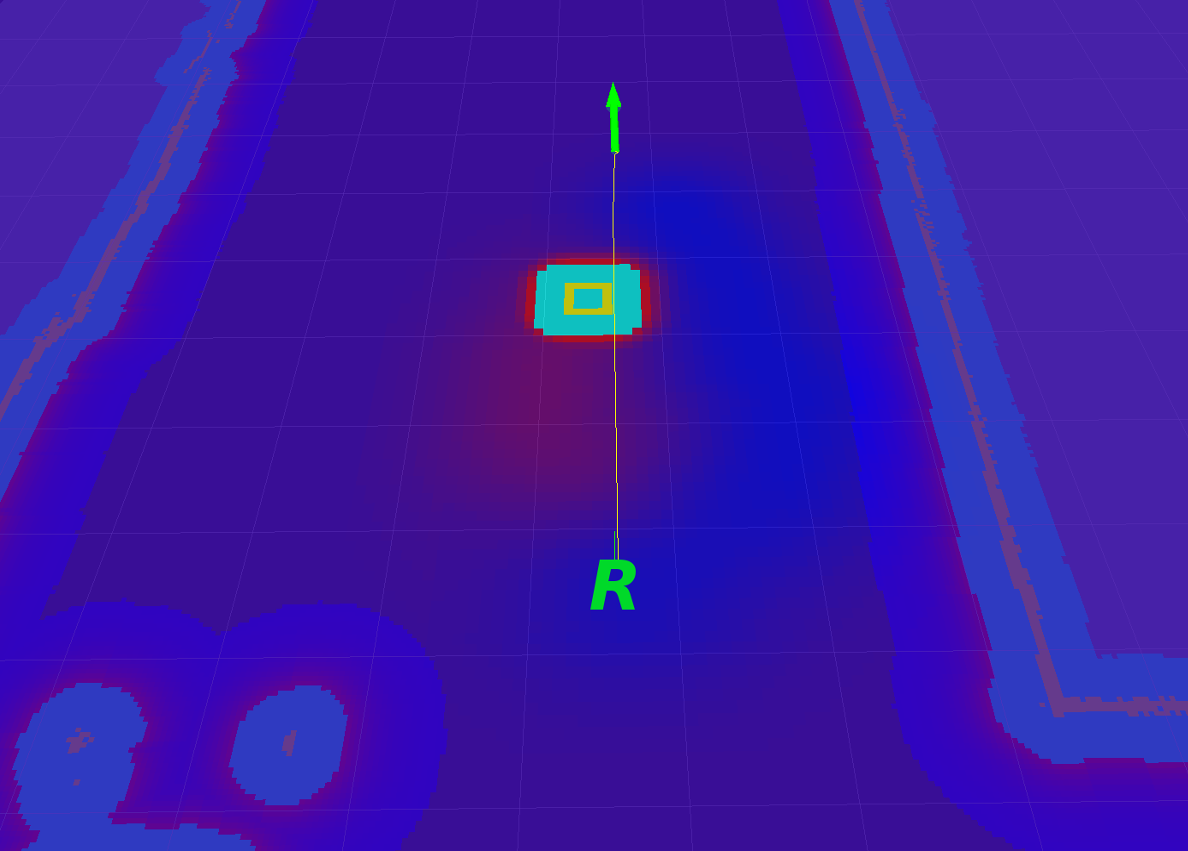
\includegraphics[height=2.8cm]{Figures/InteractiveCostmapComparison}};
		\end{tikzpicture}
	\end{center}
	
	\vspace{0.36cm}
	
	\tiny
	
	\textbf{Interactive Costmaps: Integrating Prediction and Planning with Counterfactual Reasoning}\\
	A. Bordallo, F. Previtali, S. Ramamoorthy \\
	\emph{IEEE/RSJ International Conference on Intelligent Robots and Systems, 2015} [submitted] \\
\end{frame}

\begin{frame}
	\frametitle{Quantitative Evaluation}
	\framesubtitle{InSpace}
	
	\begin{table}
		\centering
		\caption{Comparison of costmap experiments, obstacle layer is used as a baseline. CPU\% shows
				 average measured consumption and p.a. shows additional load per agent. Execution time
				 shows time required for costmap generation. Experiment times show average/worst time
				 over all trials, where $\infty s$ denotes a timeout.}
		\def\arraystretch{1.3}
		\vspace{-0.3cm}
		\resizebox{\textwidth}{!}
		{
			\begin{tabular}{lcccccc}
				Method & CPU & Execution Time & Passing Time & Crossing Time & Collisions &
				Near-collision \\ \hline
				Obstacle layer (Baseline) & -\% & -s & 5/$\infty$s & 5/$\infty$s & 80\% & 70\% \\
				Constant Velocity model & 4\%+1\% p.a. & 5ms p.a. & 15/20s & 12/18s & 40\% & 60\% \\
				Proxemics and social & 3\%+2\% p.a. & 5ms + 5ms p.a. & 8/28s & 12/14s & 20\% & 50\% \\
				\textbf{Interactive Costmap} & \textbf{6\%+2\% p.a.} & \textbf{5ms + 5ms p.a.} &
				\textbf{7/8s} & \textbf{8/9s} & \textbf{10\%} &  \textbf{20\%}  \\
			\end{tabular}
		}
	\end{table}
\end{frame}

\begin{frame}
	\frametitle{Qualitative Evaluation}
	\framesubtitle{InSpace}
	
	\begin{figure}[!h]
		\centering
		\includemovie[inline=false,text=
		{
			\begin{tikzpicture}
				\node at (0,0) [draw=black,ultra thick,inner sep=0pt]
				{
					\includegraphics[width=0.65\linewidth]{Figures/InteractiveCostmap}
				};
			\end{tikzpicture}
		}]{}{}{../Videos/3-Youbot/InteractiveCostmaps.avi}
	\end{figure}
\end{frame}

\begin{frame}
	\frametitle{Major Reviewers' Comments}
	
	\large
	
	\textbf{Rev.}\\
	``For some experiments, comparisons are only made with various versions of the same algorithms.''
	
	\vspace{0.3cm}
	
	\textbf{Rev.}\\
	``The benefits of the method are shown for activity forecasting applications, intention prediction,
	and for constructing interactive costmaps to guide robot navigation. The latter applications
	represent significant contributions in robotics. Some additional discussion of the assumptions being  
	employed would be useful. Specifically, the joint optimization seems to assume more coordination
	than, e.g., humans have when they navigate (often sub-­optimally).'' \\
\end{frame}
